\section{Resultados}

\subsection{Alineamientos de secuencias aminoacídicas de nsp10/14/16}

En relación al \href{https://htmlpreview.github.io/?https://github.com/villena-francis/bachelors_thesis/blob/main/data/align_no_ext_sp/nsp10/Trim_Alig_All_nsp10.html}{alineamiento de nsp10}, 
la baja identidad y menor longitud relativa a la secuencia del virus del salmón del Pacífico 
(PsNV) redunda en la aparición de tres regiones huecas sobre sí misma, así como 
otras dos en el resto de secuencias. Tras el proceso de depuración, 128 de 
las 150 columnas (\~{}85\%) fueron identificadas como posiciones informativas 
comparables.

Respecto al \href{https://htmlpreview.github.io/?https://github.com/villena-francis/bachelors_thesis/blob/main/data/align_no_ext_sp/nsp14/Trim_Alig_All_nsp14.html}{alineamiento de nsp14}, se observó que la 
secuencia del PsNV conserva bastantes posiciones homólogas. Sin embargo, 
también se evidenció una gran deleción que abarca las primeras 83 posiciones
del alineamiento (relativas al dominio nsp14-ExoN). Tras el proceso de 
depuración, 428 de las 567 (\~{}75\%) se identificaron como columnas 
informativas comparables.

En cuanto al \href{https://htmlpreview.github.io/?https://github.com/villena-francis/bachelors_thesis/blob/main/data/align_no_ext_sp/nsp16/Trim_Alig_All_nsp16.html}{alineamiento de nsp16}, la secuencia del 
PsNV presentó una baja cobertura respecto a las de 
\textit{Orthocoronavirinae}; queda flanqueada por dos grandes huecos que 
abarcan las regiones delimitadas por las posiciones 1--41 y 248--313. A pesar 
de ello, cabe destacar que la región abarcada por la secuencia está bastante
conservada respecto a sus homólogas. Tras el proceso de depuración, 235 de 
las 313 (\~{}85\%) se identificaron como columnas informativas comparables.

Las secuencias del PsNV, seleccionado inicialmente como especie externa, 
fueron descartadas para la reconstrucción de filogenias debido a la 
significativa ausencia de posiciones homólogas respecto a sus secuencias 
ortólogas de la subfamilia \textit{Orthocoronavirinae}. No obstante, dentro 
de dicho grupo de estudio los alineamientos de nsp10, nsp14 y nsp16 muestran
por lo general una elevada identidad de secuencia.

Los informes de depuración en HTML y los alineamientos previos en FASTA, con
las secuencias del PsNV, están para su consulta en \url{https://github.com/villena-francis/bachelors_thesis/tree/main/data/align_ext_sp}.

Los alineamientos realizados para la reconstrucción de los árboles 
filogenéticos, sin las secuencias del PsNV, están disponibles para ser 
consultados en \href{https://github.com/villena-francis/bachelors_thesis/tree/main/data/align_no_ext_sp}.

\subsection{Filogenias de nsp10/14/16 en \textit{Orthocoronavirinae}}

Los modelos evolutivos seleccionados como más apropiados para la 
reconstrucción de las filogenias fueron Q.insect+I+G4, para nsp10 y nsp14, 
y Q.insect+G4 para nsp16 (\cite{cuongbb_all_2022}). Los árboles 
filogenéticos obtenidos fueron enraizados manualmente seleccionando como 
grupo externo al género \textit{Deltacoronavirus}, en base al conocimiento 
actual de las relaciones filogenéticas de los coronavirus dentro del orden 
\textit{Nidovirales} (\cite{zhou_taxonomy_2021}).

El árbol filogenético de la familia nsp10 (\textbf{Figura 5}) muestra tres 
grupos con nodos basales bien soportados según los valores de bootstrap. Dos
de estos grupos se corresponden con los géneros \textit{Gammacoronavirus} y 
\textit{Deltacoronavirus}, mientras que en el tercero las secuencias 
pertenecientes al género Betacoronavirus forman un grupo parafilético con 
\textit{Alphacoronavirus} como grupo monofilético más reciente. 

Los árboles correspondientes a las familias nsp14 y nsp16 (\textbf{Figuras 
6} y \textbf{7}) muestran una notable similitud. En ambos casos, las 
secuencias se agrupan en cuatro clados correspondientes a cada uno de los 
géneros de la subfamilia \textit{Orthocoronavirinae}. Los nodos basales que 
los separan muestran una considerable robustez, respaldados por valores de 
bootstrap significativos.

\begin{figure}[H]
    \centering
    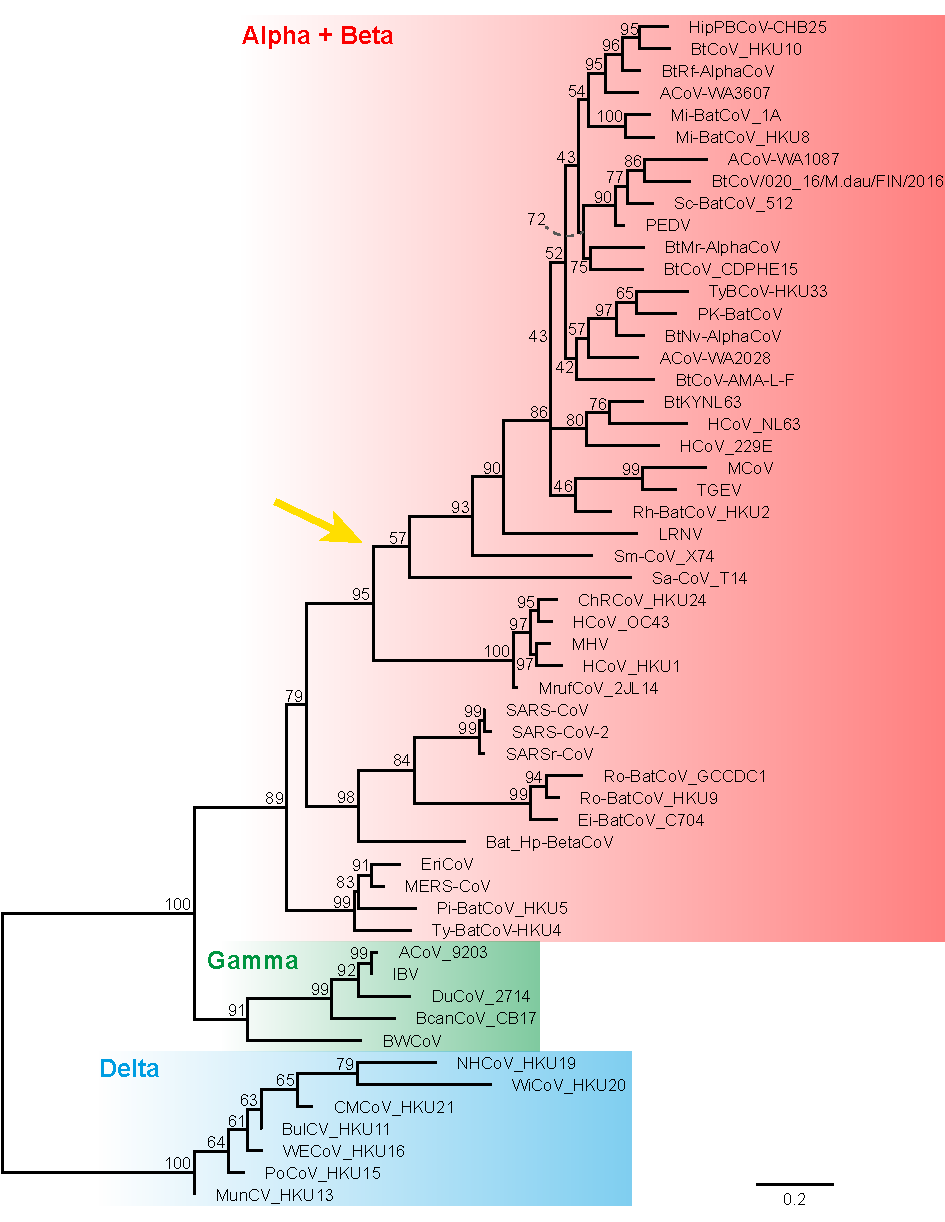
\includegraphics[width=1\textwidth]{img/fig5.pdf}
    \caption{Árbol filogenético de máxima verosimilitud de las relaciones 
    entre las proteínas nsp10 de \textit{Orthocoronavirinae}. Se destacan 
    tres grupos principales, correspondientes a los géneros
    \textit{Alphacoronavirus} + \textit{Betacoronavirus} (rojo), 
    \textit{Gammacoronavirus} (verde) y \textit{Deltacoronavirus} (cian). 
    La flecha amarilla señala la rama que aisla a todas las secuencias de 
    \textit{Alphacoronavirus} dentro de los \textit{Betacoronavirus}, y los 
    números sobre cada nodo corresponden a los valores de bootstrap. La 
    barra de la esquina inferior derecha representa en escala el número de 
    sustituciones de aminoácidos por sitio.}\label{fig:nsp10tree}
\end{figure}

\begin{figure}[H]
    \centering
    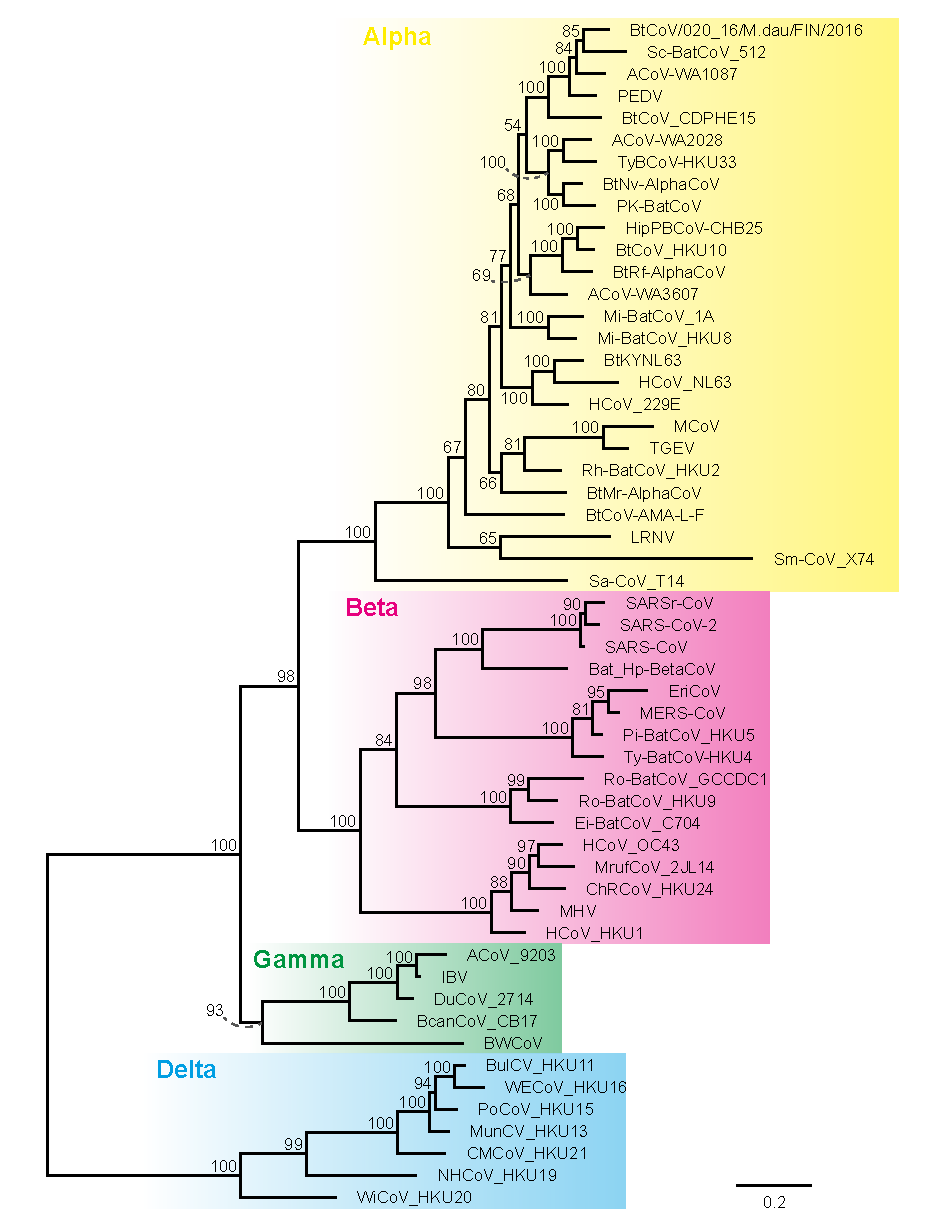
\includegraphics[width=1\textwidth]{img/fig6.pdf}
    \caption{Árbol filogenético de máxima verosimilitud de las relaciones 
    entre las proteínas nsp14 de \textit{Orthocoronavirinae}. Se destacan 
    cuatro grupos principales, correspondientes a los géneros
    \textit{Alphacoronavirus} (amarillo), \textit{Betacoronavirus}
    (magenta), \textit{Gammacoronavirus} (verde) y \textit{Deltacoronavirus} 
    (cian). Los números sobre cada nodo corresponden a los valores de 
    bootstrap y la barra de la esquina inferior derecha representa en 
    escala el número de sustituciones de aminoácidos por sitio.}\label{fig:nsp14tree}
\end{figure}

\begin{figure}[H]
    \centering
    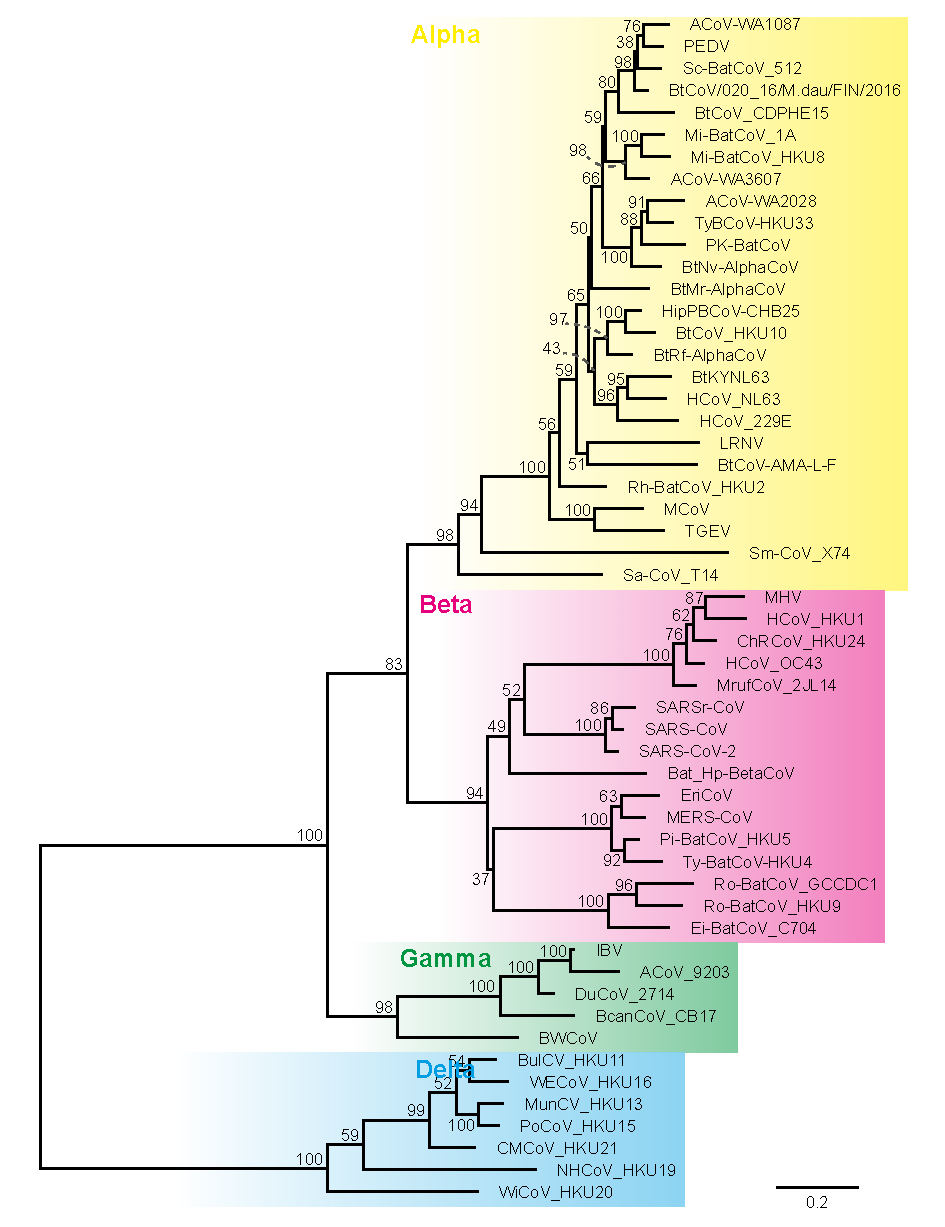
\includegraphics[width=1\textwidth]{img/fig7.pdf}
    \caption{Árbol filogenético de máxima verosimilitud que muestra las 
    relaciones entre las proteínas nsp16 de \textit{Orthocoronavirinae}. Se 
    destacan cuatro grupos principales, correspondientes a los géneros
    \textit{Alphacoronavirus} (amarillo), \textit{Betacoronavirus} (magenta),
    \textit{Gammacoronavirus} (verde) y \textit{Deltacoronavirus} (cian). 
    Los números sobre cada nodo corresponden a los valores de bootstrap, y 
    la barra de la esquina inferior derecha representa en escala el número 
    de sustituciones de aminoácidos por sitio.}\label{fig:nsp16tree}
\end{figure}

\subsection{Región de nsp10 con máxima interacción con nsp14 y nsp16}

Utilizando la estructura cristalográfica de referencia para la interacción 
nsp10/nsp14-ExoN (PDB ID:\@ 7DIY), se localizaron un total de 47 residuos de 
nsp10 que interactúan con nsp14-ExoN. Por otro lado, la estructura utilizada
como base para el estudio de la interacción (PDB ID:\@ 6W4H) reveló 22 
residuos de nsp10 interactúan con nsp16. Se encontró que de los residuos 
identificados en nsp10, 19 fueron comunes a ambas interacciones.

La región de nsp10 que muestra la mayor cantidad consecutiva de residuos
involucrados en interacciones tanto con nsp14 como con nsp16 se encuentra en
las posiciones 40--45, relativas a la secuencia aminoacídica del SARS-CoV-2. 
Sin embargo, con el objetivo de mejorar la interacción con nsp16 sin afectar
de manera significativa la interacción con nsp14, se decidió extender la 
región de interés hasta la posición 47. Estos hallazgos se presentan de 
manera gráfica en la \textbf{Figura 8A}.

La región específica de nsp10 que ha sido seleccionada se trata de una 
cadena polipeptídica extendida, es decir, que no presenta conformación 
secundaria de hélice alfa ni lámina beta. Dicho domino establece 
interacciones no covalentes con 11 residuos de nsp14-ExoN 
(\textbf{Figura 8B}), y con otros 14 residuos de nsp16 (\textbf{Figura 8C}).

Las estructuras del PDB empleadas para este los análisis de este trabajo, 
con las configuraciones de visualización y anotaciones aplicadas, están 
disponibles para su consulta en formato de sesión de ChimeraX (.cxs) en el 
siguiente enlace: \url{https://github.com/villena-francis/bachelors_thesis/tree/main/data/structures}.

\subsection{Logos de secuencias de la zona de máxima interación de nsp10 y los
dominios de nsp14 y nsp16 implicados.}

Como se muestra en la (\textbf{Figura 9}), las regiones seleccionadas de 
nsp10, nsp14-ExoN y nsp16 presentan de manera general una mayor conservación 
en el conjunto formado por \textit{Alphacoronavirus}, 
\textit{Betacoronavirus} y \textit{Gammacoronavirus}, excluyendo a 
\textit{Deltacoronavirus}. En esos tres géneros, los residuos de nsp10 
involucrados tanto en la interacción con nsp14 como nsp16 (40--45) están muy 
conservados. Sin embargo, aquellos que interactúan únicamente con nsp16 
(46--47) exhiben gran variabilidad en los cuatro géneros de 
\textit{Orthocoronavirinae}.

\newpage

\begin{figure}[H]
    \centering
    \includegraphics[width=1\textwidth]{img/fig8.pdf}
    \caption{Esquema de residuos de nsp10 (cian) involucrados en las 
    interacciones con nsp14-ExoN (magenta) y nsp16 (amarillo), resaltando 
    la región seleccionada como candidata en tonos más intensos (\textbf{A}). 
    Los aminoácidos de nsp14-ExoN y nsp16 que interactúan con esta región de 
    nsp10 se resaltan en las respectivas estructuras experimentales PDB ID:\@ 
    7DIY (\textbf{B}) y PDB ID:\@ 6W4H (\textbf{C}). La secuencia y 
    estructuras utilizadas para esta figura corresponden al SARS-CoV-2.}\label{fig:interactions}
\end{figure}

\begin{sidewaysfigure}
    \centering
    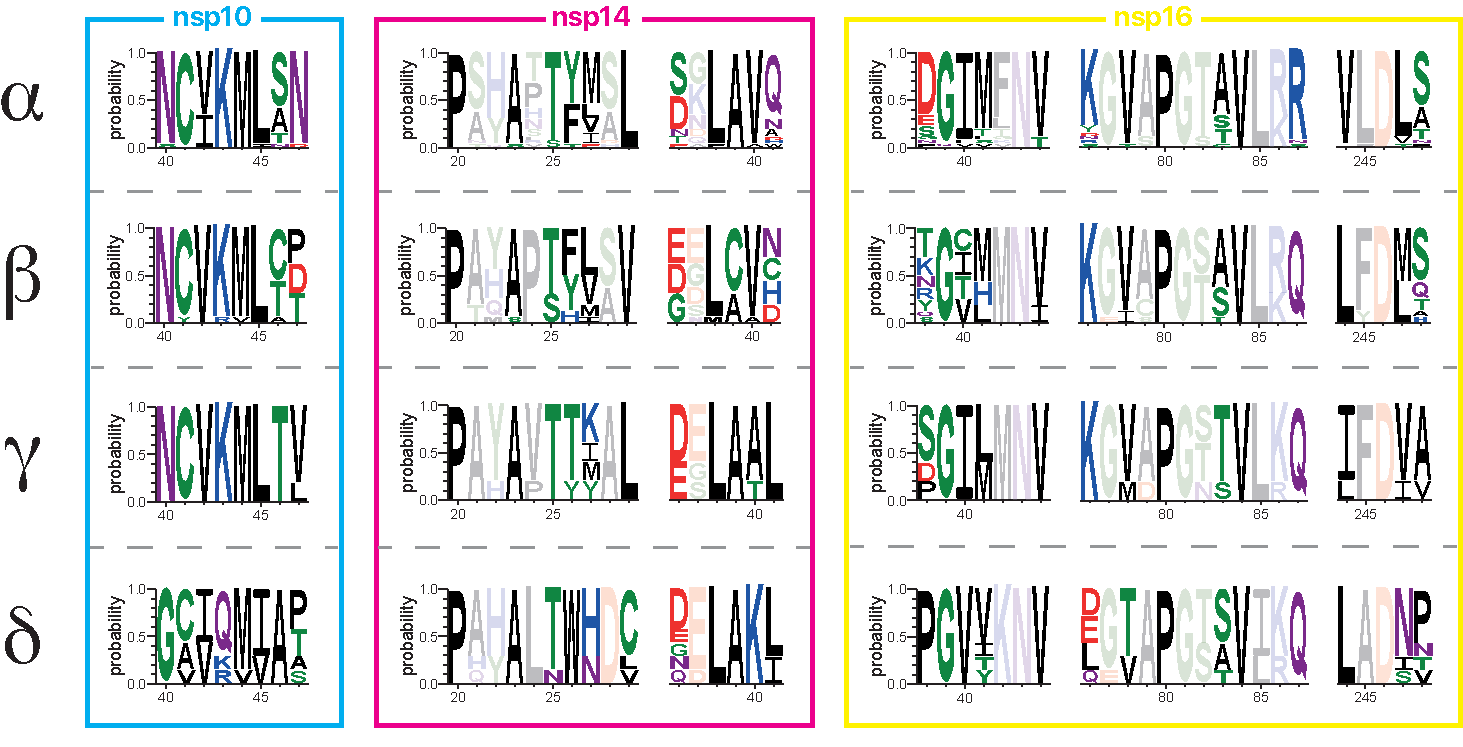
\includegraphics[width=1\textwidth]{img/fig9.pdf}
    \caption{Logos de secuencias aminoacídicas del dominio de nsp10 (cian) 
    seleccionado en este trabajo y las regiones de nsp14 (magenta) y nsp16 
    (amarillo), relativos a los géneros \textit{Alphacoronavirus}, ($\bm{\alpha}$), 
    \textit{Betacoronavirus} ($\bm{\beta}$), \textit{Gammacoronavirus} ($\bm{\gamma}$) y \textit{Deltacoronavirus} 
    ($\bm{\delta}$). Los residuos se muestran en diferentes colores: 
    hidrófobo = negro, polar = verde, básico = azul, ácido = rojo, neutro 
    = morado. Las posiciones de los residuos indicadas en el eje X se 
    corresponden a las ocupadas en las estructuras de referencia de 
    nsp10/nsp14-ExoN (PDB ID: 7DIY) y nsp10/nsp16 (PDB ID: 6W4H) empleados 
    en este trabajo. Las posiciones de nsp14 y nsp16 coloreadas débilmente 
    no intervienen en la interacción directa con residuos de nsp10.}\label{fig:logos}
\end{sidewaysfigure}

